\documentclass{article}

\usepackage[T1]{fontenc} 
\usepackage[ngerman]{babel}
\usepackage{graphicx}
\bibliography{literatur}
\usepackage{listings}

\usepackage{xcolor}
\definecolor{codegreen}{rgb}{0,0.6,0}
\definecolor{codegray}{rgb}{0.5,0.5,0.5}
\definecolor{codeorange}{rgb}{1,0.49,0}
\definecolor{backcolour}{rgb}{0.95,0.95,0.96}

\lstdefinestyle{mystyle}{
	backgroundcolor=\color{backcolour},   
	commentstyle=\color{codegray},
	keywordstyle=\color{codeorange},
	numberstyle=\tiny\color{codegray},
	stringstyle=\color{codegreen},
	basicstyle=\ttfamily\footnotesize,
	breakatwhitespace=false,         
	breaklines=true,                 
	captionpos=b,                    
	keepspaces=true,                 
	numbers=left,                    
	numbersep=5pt,                  
	showspaces=false,                
	showstringspaces=false,
	showtabs=false,                  
	tabsize=2,
	xleftmargin=10pt,
}

\lstset{style=mystyle}
	
\begin{document}
\title{Programmierung für KI \\ Projektausarbeitung - Haar Cascades}
\author{Peter, Johannes Peter, Alexander Fuchs, Onur Yilmaz}
\date{\today}
\maketitle
\newpage
	\tableofcontents
	\vspace{2cm} %Add a 2cm space

\newpage
	
\section*{Einleitung}
Im Rahmen der Veranstaltung - \textit{Programmierung für KI}, haben wir das Thema \textbf{Haar Cascades}, als gemeinsam zu bearbeitendes Projekt erhalten. Haar Cascades beschreibt ein Verfahren bzw. einen Algorithmus, welches bestimmte Merkmale oder Muster in Bildern oder Videos erkennen kann.
\\ \\
Ziel dieses Projektes ist es nun ein solches Verfahren zu implementieren und eine passende graphische Benutzeroberfläche in Python bereitzustellen. Nach einer kurzen theoretischen Einführung in das Thema, teilt sich die Arbeit in zwei Teile auf. 
Der erste Teil beschäftigt sich mit der Erstellung einer graphischen Benutzeroberfläche mit Hilfe von \textbf{Tkinter} und der zweite Teil mit \textbf{steamlit}.
\\ \\
Schrittweise werden wir auf die einzelnen Python Codes eingehen und diese näher erläutern. Des Weiteren werden wir kennzeichnen, welche Codeblock genau, welchem Projektteilnehmer zuzuordnen sind.

\section{Einführung - Haar Cascades}

Wie bereits oben erwähnt sind Haar Cascades \footnote{ Rapid object detection using a boosted cascade of simple features und Viola, Jones: Robust Real-time Object Detection, IJCV 2001, zurück zu führen auf \textit{Paul Viola} und \textit{Michael Jones}} ein Verfahren zur Erkennung von Objekten in Bildern und Videos. Genauer handelt es sich hierbei um einen Klassifikationsalgorithmus, welches Beispielbilder trainiert, die entweder das zu erkennende Muster oder Objekt enthalten oder nicht. Anschließend kann der Haar Cascade dann auf neue Bilder oder Videos angewendet werden und versucht, das gesuchte Muster oder Objekt darin wieder zu erkennen.

\subsection{Funktionsweise: Haar-like Features}
Aus den Bildern als Eingangsdaten werden so genannte Haar-like Features
als Merkmale extrahiert. Für diese Merkmale werden rechteckige Bereiche
im Bild zusammengefasst.

\begin{figure}
	\centering
	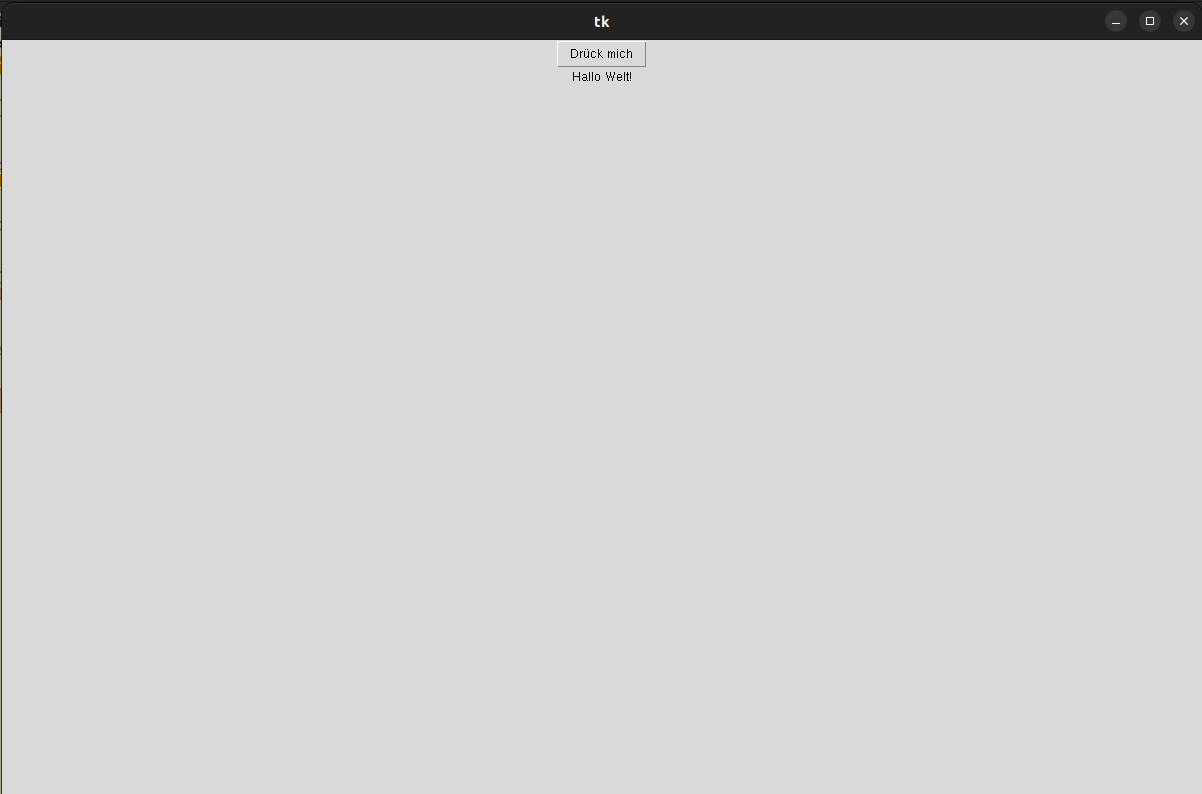
\includegraphics[width=0.7\linewidth]{foto1}
	\caption{Haar-like Features}
	\label{fig:foto1}
\end{figure}


\newpage
\subsection{Umsetzung in OpenCV}
Für unseren Anwendungsfall ist es mit Hilfe von OpenCV nicht notwendig einen eigenen Haar Cascade  Algorithmus anzulernen. Wir laden die XML-Datei mit den zugehörigen \textit{Haar-like-Features}, die wir verwenden möchten. Diese XML-Dateien enthalten Informationen darüber, wie die Features bzw. Merkmale aussehen und wie sie auf Bilder angewendet werden sollen. 



\newpage
\section{Implementation in Tkinter}
Um den Code möglichst lesbar zu gestalten, teilen wir diesen im Folgenden in mehreren kleinen Blöcke auf.
\subsection{Packages}

\begin{lstlisting}[language=Python, label = {lst:code}, mathescape= true]
import tkinter as tk
from tkinter import ttk
from tkinter import filedialog
import numpy as np
import cv2
from PIL import Image, ImageTk
import random
import os

from pki_a22_app.utils.file_loader import get_classifiers

path_haarcascade = "resources/haarcascades/haarcascade_"


classifier_list = get_classifiers()
\end{lstlisting}

%Hier schreibe auf bzgl. den wichtigsten import 
% und füge hier die requirement.txt ein

\subsection{Initialisierung und Geometrie}
\begin{lstlisting}[language=Python]
root = tk.Tk()
root.title('Projekt Gruppe a2-2 - Thema: Bilderkennung Haar-Cascades')


screen_width = root.winfo_screenwidth()
screen_height = root.winfo_screenheight()


if screen_width/screen_height < 1.8:
	window_width = int(screen_width * 0.8)
else: 
	window_width = int(screen_height * (screen_width/2/screen_height)*0.8)
	window_height = int(screen_height * 0.8)

img_max_width = int(window_width/2-75)
img_max_height = int(window_height-300) 


center_x = int(screen_width/2 - window_width / 2)
center_y = int(screen_height/2 - window_height / 2)



root.geometry(f'{window_width}x{window_height}+{center_x}+{center_y}')
root.resizable(False, False)
\end{lstlisting}

% Hier legen wir die Größe der Tkinter App fest
% Außerdem haben wir hier eine angepasste Version der Fenster Höhe/Breite für verschiedene OS

\newpage
\subsection{Bild öffnen und Klassifizierer anwenden}
\begin{lstlisting}[language=Python]
def file_open():
	global input_image
	global output_image
	filename = filedialog.askopenfilename(filetypes=(("jpg files", "*.jpg"),("png files", "*.png")))
	input_image = Image.open(filename)
	width, height = input_image.size
	aspect_ratio = width / height
	if aspect_ratio > 1:
		new_width = img_max_width
		new_height = int(new_width / aspect_ratio)
	else:  
	new_height = img_max_height
	new_width = int(new_height * aspect_ratio)
	input_image = input_image.resize((new_width,new_height), Image.ANTIALIAS)
	input_image_tk = ImageTk.PhotoImage(input_image)
	input_img_label.config(image=input_image_tk)
	input_img_label.image = input_image_tk

	output_image = Image.open(filename)
	output_image = output_image.resize((new_width,new_height), Image.ANTIALIAS)
	output_image_tk = ImageTk.PhotoImage(output_image)
	output_img_label.config(image=output_image_tk)
	output_img_label.image = output_image_tk
\end{lstlisting}

% Funktionen um ein beliebiges Bild im png oder jpg Format zu öffnen
% (aspect_ratio) --> Anzeige des Bildes erfolgt im richtigen Seitenverhältnis, erneut
% angepasst an der Fensterbreite und Höhe


\begin{lstlisting}[language=Python]
def img_change(classifier):
	global input_image
	global output_image
	cascade = cv2.CascadeClassifier(path_haarcascade + classifier + ".xml")
	output_image_cv = np.array(output_image.convert('RGB'))
	output_image_cv_gray = cv2.cvtColor(output_image_cv, cv2.COLOR_BGR2GRAY)
	cascade_results = cascade.detectMultiScale(output_image_cv_gray, scaleFactor=s1.get_val(), minNeighbors = s2.get_val(), minSize=(s3.get_val(), s3.get_val())) 
	iterations = 0

	if len(cascade_results) > 0:
		color = (random.randint(0,255),random.randint(0,255),random.randint(0,255))
		for (x,y,w,h) in cascade_results:
			cv2.rectangle(output_image_cv,(x,y),(x+w,y+h),(color),2)
			roi_gray = output_image_cv_gray[y:y+h, x:x+w]
			roi_color = output_image_cv[y:y+h, x:x+w]
		output_image = Image.fromarray(output_image_cv) 
		output_img_label.image.paste(output_image)
	else:
		flag = False
		for i1 in np.arange (1.5, 0.9, -0.1):
			for i2 in range (6, 2, -1):
				for i3 in range (50, 9, -10):                 
					s1.s.set(i1)
					s2.s.set(i2)
					s3.s.set(i3)
					iterations = iterations + 1
					cascade_results = cascade.detectMultiScale(output_image_cv_gray, scaleFactor=s1.get_val(), minNeighbors = s2.get_val(), minSize=(s3.get_val(), s3.get_val()))
					if len(cascade_results) > 0:
						color = (random.randint(0,255),random.randint(0,255),random.randint(0,255))
						for (x,y,w,h) in cascade_results:
							cv2.rectangle(output_image_cv,(x,y),(x+w,y+h),(color),2)
							roi_gray = output_image_cv_gray[y:y+h, x:x+w]
							roi_color = output_image_cv[y:y+h, x:x+w]
							output_image = Image.fromarray(output_image_cv)
							output_img_label.image.paste(output_image)
							flag = True
							break
					if flag: break
				if flag: break
			if len(cascade_results) == 0:
				print(f"Kein Ergebnis nach {iterations} Iterationen")          
\end{lstlisting}



\begin{lstlisting}[language=Python]
def output_image_restart():
	global input_image
	global output_image
	output_image = input_image
	output_img_label.image.paste(output_image)
\end{lstlisting}


\subsection{Slider und Button}
\begin{lstlisting}[language=Python]
class slider:    
	def __init__(self,name,x_pos=0,y_pos=0,scale_from=0,scale_to=100,typ=int):
		self.name = name
		self.x_pos = x_pos
		self.y_pos = y_pos
		self.scale_from = scale_from
		self.scale_to = scale_to
		if typ==int: 
			self.val = tk.IntVar() 
		else: 
			self.val = tk.DoubleVar() 

		self.lbl = ttk.Label(root, text=name)
		self.lbl.place(x=self.x_pos,y=self.y_pos)

		self.s = ttk.Scale(root, from_=self.scale_from, to=self.scale_to, 	orient="horizontal",command=self.slider_change,variable=self.val)
		self.s.place(x=self.x_pos+100,y=self.y_pos)

		self.v = ttk.Label(root,text=f"{self.get_val():.1f}")
		self.v.place(x=self.x_pos+210,y=self.y_pos)
	def get_val(self):
		return self.val.get()
	def slider_change(self, event):
		self.v.configure(text=f"{self.get_val():.1f}")
\end{lstlisting}

% da nicht absehbar war, wie viele Slider am Ende benutzt wurde hier eine Klasse verwendet.


\begin{lstlisting}[language=Python]
def blur_rectangle(classifier):
	global input_image
	global output_image
	cascade = cv2.CascadeClassifier(path_haarcascade + classifier + ".xml")
	output_image_cv = np.array(output_image.convert('RGB'))
	output_image_cv_gray = cv2.cvtColor(output_image_cv, cv2.COLOR_BGR2GRAY)
	cascade_results = cascade.detectMultiScale(output_image_cv_gray, scaleFactor=s1.get_val(), minNeighbors = s2.get_val(), minSize=(s3.get_val(), s3.get_val()))
		if len(cascade_results) > 0:
			for (x,y,w,h) in cascade_results:
				face = output_image_cv[y:y+h, x:x+w]
				face = cv2.GaussianBlur(face, (23, 23), 30)
				output_image_cv[y:y+h, x:x+w] = face

			output_image = Image.fromarray(output_image_cv)
			output_img_label.image.paste(output_image)

def save_jpg():
	file_path = filedialog.asksaveasfilename(initialfile="output_image", filetypes=(("jpg files", "*.jpg"),("png files", "*.png")), defaultextension=".jpeg")
	if file_path:
		output_image.save(file_path)

tk.Button(root, text="Bild aus Datei oeffnen", command=file_open).place(x=window_width/2-window_width/4,y=150)
tk.Button(root, text="Classifier anwenden", command=lambda: img_change(dropdown.get())).place(x=window_width/2+window_width/4,y=150)
tk.Button(root, text="==>", command=output_image_restart).place(x=window_width/2-12.5,y=window_height/2)
tk.Button(root, text="Weichzeichnen",command=lambda: blur_rectangle(dropdown.get())).place(x=window_width/2+window_width/4+122,y=150)
tk.Button(root, text="Bild speichern",command=save_jpg).place(x=window_width/2+window_width/4+220,y=150)

dropdown = tk.StringVar(root)
dropdown.set(classifier_list[2])
dropdown_label = tk.OptionMenu(root, dropdown, *classifier_list)
dropdown_label.place(x=window_width/2-75,y=20)


xpos_slider_window = window_width/2 -75
ypos_slider_window = 60
s1 = slider("ScaleFactor",xpos_slider_window,ypos_slider_window,1.01,1.5,float)
s1.s.set(1.1)
s2 = slider("MinNeighbors",xpos_slider_window,ypos_slider_window+30,3,6)
s2.s.set(4)
s3 = slider("minSize",xpos_slider_window,ypos_slider_window+60,10,50)
s3.s.set(30)


input_img_label = ttk.Label(root)
input_img_label.place(x=25,y=200)

output_img_label = ttk.Label(root)
output_img_label.place(x=window_width/2+50,y=200)

fh_logo = Image.open("resources/images/Logo.jpg")
fh_logo = fh_logo.resize((300,100), Image.ANTIALIAS)
fh_logo_tk = ImageTk.PhotoImage(fh_logo)
ttk.Label(root, image=fh_logo_tk).place(x=0,y=0)

root.mainloop()	
\end{lstlisting}







\newpage
\section{Implementation in Streamlit}
\end{document}
